% Generated by fig_progressive.py; edit the script, not this file.
\documentclass[border=0pt]{standalone}
\usepackage[T1]{fontenc}
\usepackage{times}
\usepackage{graphicx}
\usepackage{tikz}
\graphicspath{{../progressive/}}
% Written by scafig.py; the same palette as the matplotlib figures.
\definecolor{scaInk}{HTML}{1F2328}
\definecolor{scaMid}{HTML}{5B6570}
\definecolor{scaRule}{HTML}{C3C9CF}
\definecolor{scaGrid}{HTML}{E6E9EC}
\definecolor{scaGlobal}{HTML}{2F6DB3}
\definecolor{scaGlobalLight}{HTML}{DCE7F3}
\definecolor{scaLocal}{HTML}{E08A2B}
\definecolor{scaLocalLight}{HTML}{F9E6D0}
\definecolor{scaAccent}{HTML}{13865F}
\definecolor{scaAccentLight}{HTML}{D7EEE4}
\definecolor{scaNeutral}{HTML}{F4F1EA}
\definecolor{scaZoom}{HTML}{FFC21A}
\definecolor{scaLoss}{HTML}{B85C00}
\definecolor{scaArea}{HTML}{7A4EA3}
\definecolor{scaAreaLight}{HTML}{E9E0F1}
\definecolor{scaFull}{HTML}{9AA3AC}

\begin{document}
\begin{tikzpicture}[x=1in,y=1in,
  halo/.style={draw=black,draw opacity=0.35,line width=1.1pt},
  zoombox/.style={draw=scaZoom,line width=0.55pt},
  cropframe/.style={draw=scaZoom,line width=0.5pt},
  head/.style={font=\sffamily\fontsize{8.5}{10}\selectfont,text=scaInk},
  headours/.style={font=\sffamily\fontsize{8.5}{10}\selectfont,text=scaAccent}]
\useasboundingbox (0,0) rectangle (5.5000,-1.9267);
\node[anchor=north west,inner sep=0pt] at (0.0000,-0.1500) {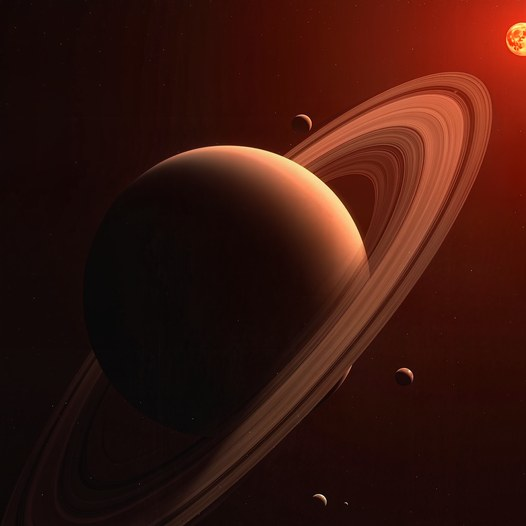
\includegraphics[width=0.8758in,height=0.8758in]{cmp_minus5023570400257826529_hrdit_dev_author.jpg}};
\draw[halo] (0.4944,-0.4887) rectangle (0.6038,-0.5982);
\draw[zoombox] (0.4944,-0.4887) rectangle (0.6038,-0.5982);
\node[anchor=north west,inner sep=0pt] at (0.9008,-0.1500) {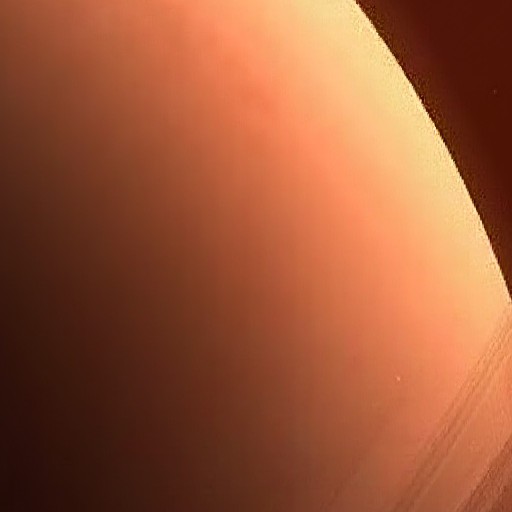
\includegraphics[width=0.8758in,height=0.8758in]{cmp_minus5023570400257826529_hrdit_dev_author_crop.jpg}};
\draw[cropframe] (0.9008,-0.1500) rectangle (1.7767,-1.0258);
\node[anchor=north west,inner sep=0pt] at (1.8617,-0.1500) {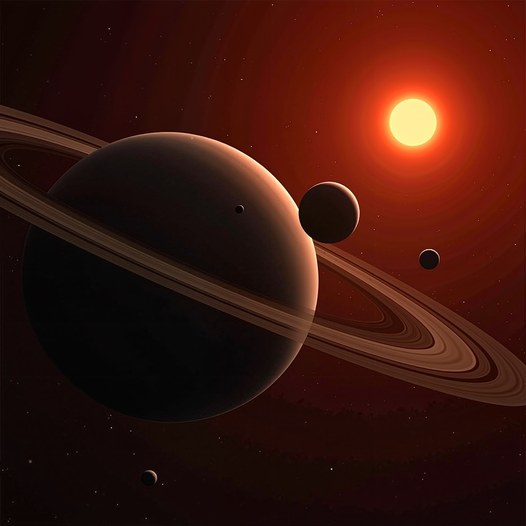
\includegraphics[width=0.8758in,height=0.8758in]{cmp_minus5023570400257826529_sca_prog.jpg}};
\draw[halo] (2.3560,-0.4887) rectangle (2.4655,-0.5982);
\draw[zoombox] (2.3560,-0.4887) rectangle (2.4655,-0.5982);
\node[anchor=north west,inner sep=0pt] at (2.7625,-0.1500) {
\includegraphics[width=0.8758in,height=0.8758in]{cmp_minus5023570400257826529_sca_prog_crop.jpg}};
\draw[cropframe] (2.7625,-0.1500) rectangle (3.6383,-1.0258);
\node[anchor=north west,inner sep=0pt] at (3.7233,-0.1500) {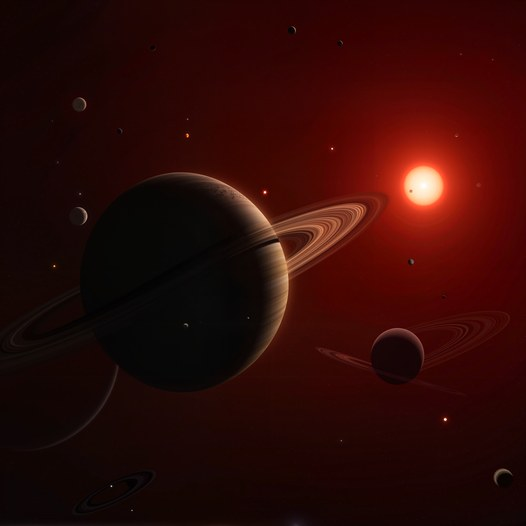
\includegraphics[width=0.8758in,height=0.8758in]{cmp_minus5023570400257826529_sca_nb.jpg}};
\draw[halo] (4.2177,-0.4887) rectangle (4.3272,-0.5982);
\draw[zoombox] (4.2177,-0.4887) rectangle (4.3272,-0.5982);
\node[anchor=north west,inner sep=0pt] at (4.6242,-0.1500) {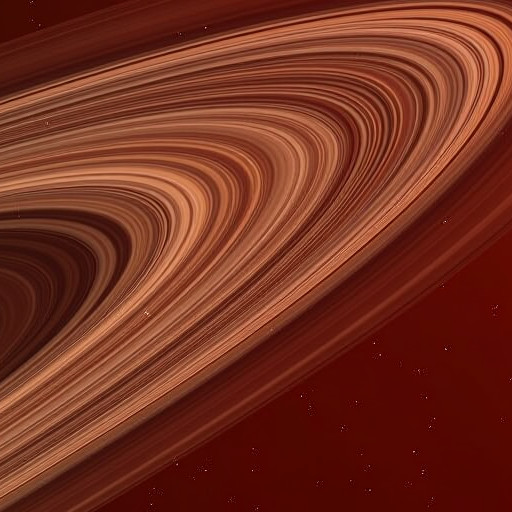
\includegraphics[width=0.8758in,height=0.8758in]{cmp_minus5023570400257826529_sca_nb_crop.jpg}};
\draw[cropframe] (4.6242,-0.1500) rectangle (5.5000,-1.0258);
\node[anchor=north west,inner sep=0pt] at (0.0000,-1.0508) {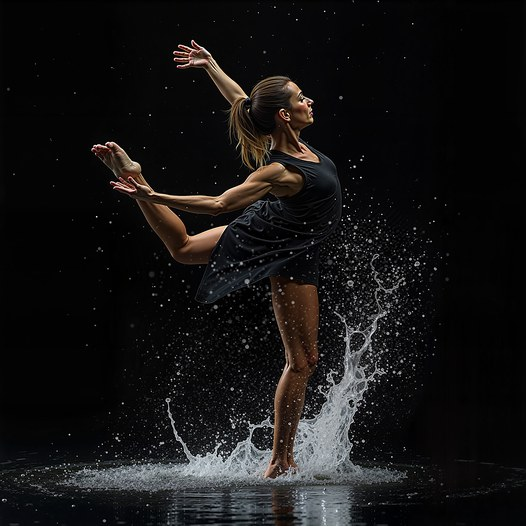
\includegraphics[width=0.8758in,height=0.8758in]{cmp_minus2679953061215100202_hrdit_dev_author.jpg}};
\draw[halo] (0.2823,-1.7436) rectangle (0.3917,-1.8531);
\draw[zoombox] (0.2823,-1.7436) rectangle (0.3917,-1.8531);
\node[anchor=north west,inner sep=0pt] at (0.9008,-1.0508) {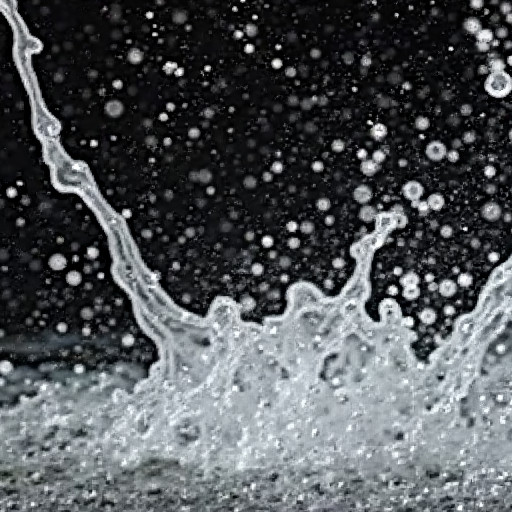
\includegraphics[width=0.8758in,height=0.8758in]{cmp_minus2679953061215100202_hrdit_dev_author_crop.jpg}};
\draw[cropframe] (0.9008,-1.0508) rectangle (1.7767,-1.9267);
\node[anchor=north west,inner sep=0pt] at (1.8617,-1.0508) {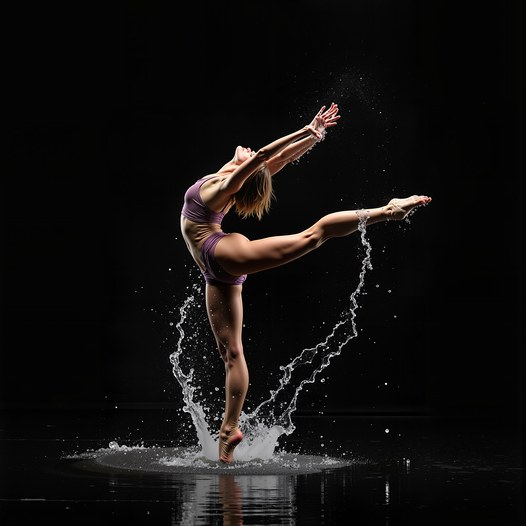
\includegraphics[width=0.8758in,height=0.8758in]{cmp_minus2679953061215100202_sca_prog.jpg}};
\draw[halo] (2.1439,-1.7436) rectangle (2.2534,-1.8531);
\draw[zoombox] (2.1439,-1.7436) rectangle (2.2534,-1.8531);
\node[anchor=north west,inner sep=0pt] at (2.7625,-1.0508) {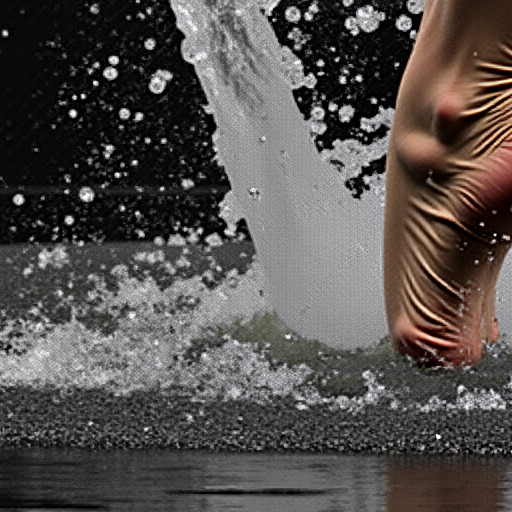
\includegraphics[width=0.8758in,height=0.8758in]{cmp_minus2679953061215100202_sca_prog_crop.jpg}};
\draw[cropframe] (2.7625,-1.0508) rectangle (3.6383,-1.9267);
\node[anchor=north west,inner sep=0pt] at (3.7233,-1.0508) {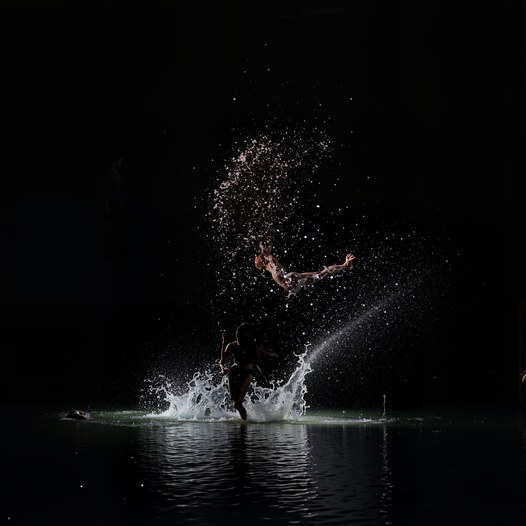
\includegraphics[width=0.8758in,height=0.8758in]{cmp_minus2679953061215100202_sca_nb.jpg}};
\draw[halo] (4.0056,-1.7436) rectangle (4.1151,-1.8531);
\draw[zoombox] (4.0056,-1.7436) rectangle (4.1151,-1.8531);
\node[anchor=north west,inner sep=0pt] at (4.6242,-1.0508) {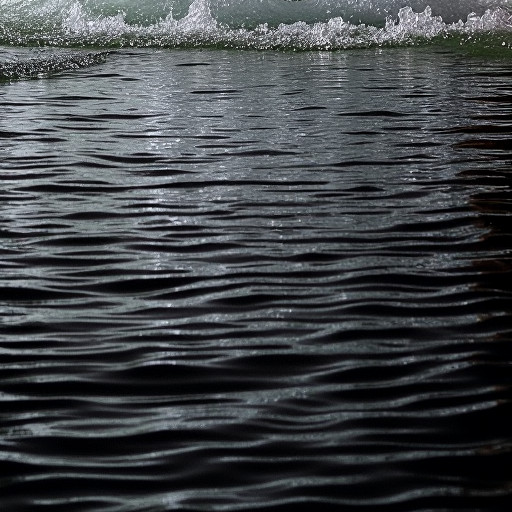
\includegraphics[width=0.8758in,height=0.8758in]{cmp_minus2679953061215100202_sca_nb_crop.jpg}};
\draw[cropframe] (4.6242,-1.0508) rectangle (5.5000,-1.9267);
\node[head,anchor=base] at (0.8883,-0.1050) {HRDiT, 106.5\,s};
\node[headours,anchor=base] at (2.7500,-0.1050) {\textbf{Progressive SCA (ours), 49.0\,s}};
\node[headours,anchor=base] at (4.6117,-0.1050) {SCA, single pass (ours), 71.6\,s};
\end{tikzpicture}
\end{document}
